We describe on this section the implementation of the Calling Context Tree in TraceCompass, the Flame Graph comparison, and the Auto cluster mechanism.

The CCT View is an analysis developed in TraceCompass framework \cite{tracecompass}, which specifically aims to study the CCT and its variations. The module with Auto clustering was included on it. The view displays the calling functions in a graphic view that helps the developer/tester to improve their codes and to compare the traces using the approach described on this work.\\

\textbf{\textit{Tree Construction}}\\
The CCT View builds the tree from the tracing as explained in the section Tree Construction. In summary the tracing is read in order and event entry-exit pairs are grouped in nodes, sub-nodes are defined by pairs of entry-exit inside the above node. The data found, i.e the performance metrics, of the nodes is summarized for the respective node. The tree is build to summarized the redundant nodes, thus, avoiding the build of a Dynamic Call Tree. Figure \ref{fig:cct_view}, shows this feature in the CCT View.\\
    
 \begin{figure*}[h]
  \centering
    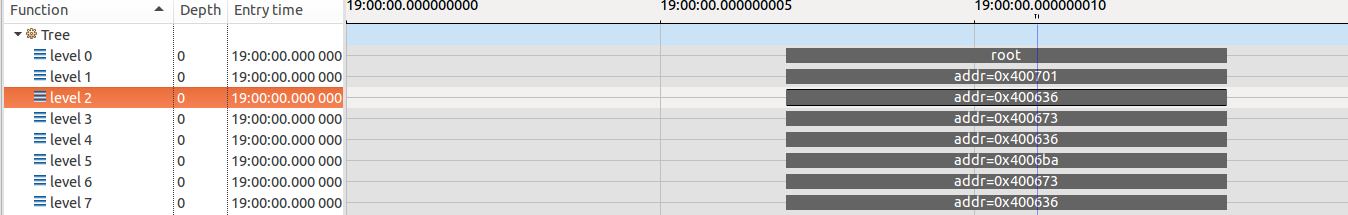
\includegraphics[width=2\columnwidth]{figures/cct_view.png}
    \caption{CCT View in TraceCompass }
    \label{fig:cct_view}
\end{figure*}

\textbf{\textit{Differential Flame Graph}}\\
The CCT View implements a Differential Flame Graph view to compare executions and groups of executions. Usually the Differential Flame Graph compares two executions, but on our implementation it is possible to compare groups of executions. In our implementation the flame graphs are composed of three colors: green (to represent equals amount of time), red (slower executions) and gray (faster executions). 

Figure \ref{fig:flame}, shows a diagram of the RGG Differential Flame Graph, the green color shows the functions which are faster in the main execution, the grey part means they are equal and the red part means that this function is slower with the comparative one. The name, RGG flamegraph brings allusion of this concept in contrast with Brendan Gregg's Red/Blue Flame Graph. 
 
 \begin{figure}[h]
  \centering
    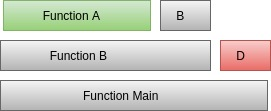
\includegraphics[width=0.5\textwidth]{figures/flame.jpg}
  \caption{RGG Differential Flame Graph Diagram}
  \label{fig:flame}
\end{figure}

\textbf{\textit{Auto cluster}}\\
The Auto cluster feature was implemented on CCT View to help developers execute similar performance cause analysis on tracing. The heuristic evaluation (elbow method) and the clustering techniques (k-means and percentage clustering) were implemented separately, therefore the developer can choose the most suitable one.\\
    
\textbf{\textit{Correlation feature}}\\
Another feature of the CCT View is the possibility to find the correlation matrix of the metrics. 
As the dictum states, "correlation does not imply causation", which means that correlation by itself cannot be used to infer a causal relationship between the studied variables.
    